\documentclass{article}\usepackage[]{graphicx}\usepackage[]{xcolor}
% maxwidth is the original width if it is less than linewidth
% otherwise use linewidth (to make sure the graphics do not exceed the margin)
\makeatletter
\def\maxwidth{ %
  \ifdim\Gin@nat@width>\linewidth
    \linewidth
  \else
    \Gin@nat@width
  \fi
}
\makeatother

\definecolor{fgcolor}{rgb}{0.345, 0.345, 0.345}
\newcommand{\hlnum}[1]{\textcolor[rgb]{0.686,0.059,0.569}{#1}}%
\newcommand{\hlsng}[1]{\textcolor[rgb]{0.192,0.494,0.8}{#1}}%
\newcommand{\hlcom}[1]{\textcolor[rgb]{0.678,0.584,0.686}{\textit{#1}}}%
\newcommand{\hlopt}[1]{\textcolor[rgb]{0,0,0}{#1}}%
\newcommand{\hldef}[1]{\textcolor[rgb]{0.345,0.345,0.345}{#1}}%
\newcommand{\hlkwa}[1]{\textcolor[rgb]{0.161,0.373,0.58}{\textbf{#1}}}%
\newcommand{\hlkwb}[1]{\textcolor[rgb]{0.69,0.353,0.396}{#1}}%
\newcommand{\hlkwc}[1]{\textcolor[rgb]{0.333,0.667,0.333}{#1}}%
\newcommand{\hlkwd}[1]{\textcolor[rgb]{0.737,0.353,0.396}{\textbf{#1}}}%
\let\hlipl\hlkwb

\usepackage{framed}
\makeatletter
\newenvironment{kframe}{%
 \def\at@end@of@kframe{}%
 \ifinner\ifhmode%
  \def\at@end@of@kframe{\end{minipage}}%
  \begin{minipage}{\columnwidth}%
 \fi\fi%
 \def\FrameCommand##1{\hskip\@totalleftmargin \hskip-\fboxsep
 \colorbox{shadecolor}{##1}\hskip-\fboxsep
     % There is no \\@totalrightmargin, so:
     \hskip-\linewidth \hskip-\@totalleftmargin \hskip\columnwidth}%
 \MakeFramed {\advance\hsize-\width
   \@totalleftmargin\z@ \linewidth\hsize
   \@setminipage}}%
 {\par\unskip\endMakeFramed%
 \at@end@of@kframe}
\makeatother

\definecolor{shadecolor}{rgb}{.97, .97, .97}
\definecolor{messagecolor}{rgb}{0, 0, 0}
\definecolor{warningcolor}{rgb}{1, 0, 1}
\definecolor{errorcolor}{rgb}{1, 0, 0}
\newenvironment{knitrout}{}{} % an empty environment to be redefined in TeX

\usepackage{alltt}

\usepackage{algorithm}
\usepackage{algpseudocode}

\usepackage{amsthm}
\usepackage{amsmath}
\usepackage{amsfonts}

\newtheorem{lemma}{Lemma}
\newtheorem{exercise}{Exercise}
\newtheorem{example}{Example}
\newtheorem{theorem}{Theorem}
\newtheorem{corollary}{Corollary}


\title{Computational Statistics, M1 MAS DS, Aix-Marseille University}
\author{Houssam BOUKHECHAM}
\IfFileExists{upquote.sty}{\usepackage{upquote}}{}
\begin{document}

\maketitle
\tableofcontents
% Here is an example R code:

% <<echo=TRUE>>=
% x <- c(1, 2, 3, 4, 5)
% mean(x)
% @

\newpage
%%%%%%%%%%%%
\section{Random variable simulation}

% TODO: A small introduction 
\cite{RobertCasela1999MonteCarloSM, gentle2009computational, tokdar2010importance}

\subsection{Transformation methods}

\begin{lemma}
  Let $F:\mathbb{R} \to [0,1]$ be an non-decreasing function. 
  If a random variable $X$ has $F$ as its cumulative distribution function (CDF), then the random variable $U = F(X) \sim U(0,1)$.
\end{lemma}
  
\begin{proof}
  % TODO
\end{proof}


\begin{example}[Normal variable generation]

  The cumulative distribution function (CDF) of a Gaussian random variable with mean $\mu$ and standard deviation $\sigma$ is given by:  
  \begin{equation}\label{CDF of a Gaussian(mu,sigma)}
  F(x) = \frac{1}{\sqrt{2\pi\sigma^2}} \int_{-\infty}^x e^{-\frac{1}{2}\left(\frac{t-\mu}{\sigma}\right)^2}~dt.
  \end{equation}  
  The function $F$ is a diffeomorphism. Assuming $\mu = 0$ and $\sigma = 1$, an approximation $F_a^{-1}$ of the inverse function $F^{-1}$ can be computed to arbitrary precision (\cite{see RC MCSM}, Example 2.6). To generate a random sample of size $n$ from the standard Gaussian distribution, we first generate $n$ random samples from the uniform distribution, $\{u_1, u_2, \ldots, u_n\}$. Then, we map this sample to the Gaussian distribution using the inverse approximation :  
  \[
  \left\{F_a^{-1}(u_1), F_a^{-1}(u_2), \ldots, F_a^{-1}(u_n)\right\}.
  \]
  
  \end{example}
  
  \begin{exercise}
  \begin{enumerate}
  \item[] 
  \item Generate a sample $\mathcal{S} = \left\{u_1, u_2, \cdots, u_n\right\}$ of size $n = 500$ from the uniform distribution.
  
  \item Implement the function
  \[
  F_a^{-1}(u) = t - \frac{a_0 + a_1t}{1+b_1t+b_2t^2}, \quad u\in(0,1),
  \]
  where $t^2 = \log\left(u^{-2}\right)$ and $a_0 = 2.30753, a_1 = 0.27061, b_1 = 0.99229, b_2 = 0.04481$
  
  \item Plot the histogram of the set $F_a^{-1}(\mathcal{S})$ and comment the results.
  
  \item$\clubsuit$ Repeat the process for a larger value of $n$ (e.g., $n = 50000$). Compare the generated sample with a standard Gaussian random variable generator and comment the results.
  
  \end{enumerate}
  \end{exercise}


\begin{exercise}

\begin{enumerate}
\item[]
\item Assume we can simulate $\mathcal{N}(0,1)$, how to generate a sample from $\mathcal{N}(\mu,\sigma^2)$?
\item Implement this method in R or Python.
\end{enumerate}

\end{exercise}

\begin{exercise}

Let $\lambda>0$ and $U$ be a random variable uniformly distributed on the interval $[0,1]$.
\begin{enumerate}
\item Prove that the random variable defined by $X = -\frac{\log(U)}{\lambda}$ follows an exponential distribution with scale parameter $\lambda$, denoted as $\mathcal{E}xp(\lambda)$.
\item Using the uniform distribution and the result from the previous question, generate a sample of size $n=100$ from $\mathcal{E}xp(1)$.
\item Compare the generated sample with a sample produced by a function in R or Python.
\end{enumerate}
\end{exercise}

\begin{exercise}
Let $N$ be a random variable with a Poisson distribution $\mathcal{P}(\lambda)$, and let $X_i$ be i.i.d. random variables with an $\mathcal{E}xp(\lambda)$ distribution.
\begin{enumerate}
\item Prove that 
\begin{equation*}
Pr(N = k) = Pr(X_1+\cdots+X_k \leq 1 < X_1 + \cdots + X_{k+1}).
\end{equation*}
\item Using the previous question, outline the steps to simulate a Poisson distribution $\mathcal{P}(\lambda)$, and then implement your algorithm in R or Python.
\item $\clubsuit$ Do you recommend this method when $\lambda$ is large ?
\end{enumerate}
\end{exercise}

\begin{exercise}
\begin{enumerate}
\item[]
\item Sketch how to generate a discrete random variable using the uniform distribution.
\item Generate a sample of size 30 from the binomial distribution with 10 trials and a success rate of 0.3, denoted by $B(n,p)$, where $n = 10$ and $p = 0.3$.
\end{enumerate}
\end{exercise}

%%%
\subsection{Accept-reject method}
In the previous subsection, we discussed how to generate Gaussian and exponential distributions from a uniform distribution, but in doing so, we needed an approximation of the inverse of the CDF. In general, the analytic form of the inverse of the CDF is not available, and even if the analytic form exists, approximation of this function may be computationally expensive. An alternative to transformation methods, is the \textit{Accept-Reject} method.
Roughly speaking, this method is a technique for generating a sample from a target distribution with density $f$, when direct sampling from it is not possible. Instead, we use a proposal distribution with density $g$, from which we generate $x$, and depending on the values of $g(x)$ and $f(x)$, we either accept $x$ as a sample of $f$ or reject it. More precisely if $f$ has a compact support and is bounded then we have 


\begin{theorem}[Fundamental theorem of simulation]\label{Fundamental theorem of simulation}
Let $f$ be a target density. Then simulating $X\sim f$ is equivalent to simulating 
\begin{equation}\label{Fund thm of sim eq}
\left(X, U\right) \sim \mathcal{U}\left\{(x,u)~:~0< u < f(x)\right\}.
\end{equation}

\end{theorem}

To simulate $X \sim f$, we first choose a value $M$ bigger than the maximum of $f$. Next, we generate a pair $(x, u)$ from a uniform distribution over the rectangle $[a, b] \times [0, M]$, where $[a,b]$ is the support of $f$. The value $x$ is accepted if $u \leq f(x)$; otherwise, it is rejected.



\begin{example}[Generation of Beta($2,4$) sample] The target density $f$ of $Beta(2,4)$ is given by 
\begin{equation}\label{Target_density_Beta}
f(x) =
\begin{cases} 
20 x(1-x)^3, & \text{if } x \in (0,1), \\ 
0, & \text{otherwise}.
\end{cases}
\end{equation}

So, if we take $M=\frac{11}{5}$, then $f\leq M.$ If we apply the Accept-Reject algorithm  for 1000 iteration, we get Figure \ref{fig:GeneratingBetaDistr}.

\begin{figure}[h]
    \centering
    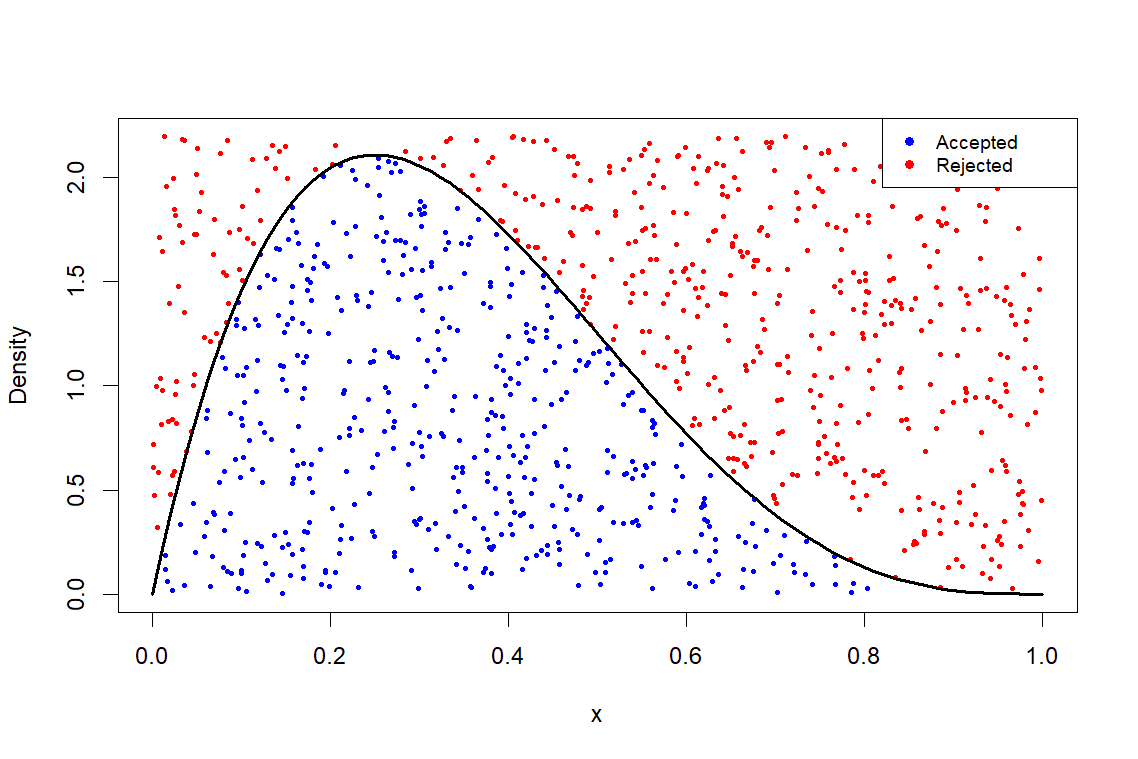
\includegraphics[width=0.8\textwidth]{Figures/Accept-Reject generation of a Beta sample.png}
    \caption{Generating Beta(2,4) using the Accept-Reject method. The Red point are rejected, while the blue ones are accepted.}
    \label{fig:GeneratingBetaDistr}
\end{figure}

\end{example}

% Generating Beta distribution
\begin{exercise}
\begin{enumerate}
\item[]
\item Using the \textit{Accept-Reject} method, generate a sample of size $n = 1000$.
\item How many iteration do we need on average to generate $n$ sample ?
\end{enumerate}
\end{exercise}

Now, if we assume that the target density does not have a compact support ($f$ is equal to zero outside an interval $[a,b]$), then we can't apply the previous technique. So we have to bound $f$ by a distribution $g$ which we can sample from (for example a Normal distribution), more precisely Theorem \ref{Fundamental theorem of simulation} implies 

\begin{corollary}\label{Accept-reject theo corr}
Let $f$ be a target density and $g$ a density which we can sample from. Assume that there is $M\in \mathbb{R}$ such that 
\begin{equation*}
f(x) \leq M g(x), ~\forall x.
\end{equation*}

Then to simulate $X \sim f$, we simulate 
\begin{equation*}
Y \sim g,\quad U|Y \sim \mathcal{U}\big(0,M\cdot g(Y)\big),
\end{equation*}
until $ u < f(y)$.
\end{corollary}

Using Corollary \ref{Accept-reject theo corr}, the Accept-Reject method can be done as follows

\begin{algorithm}[H]
\caption{Accept-Reject}
\label{alg:accept-reject}
\begin{algorithmic}[1]
\State Choose \( M \geq 1 \) such that \( f(x) \leq M g(x) \) for all \( x \).
\State \label{step:generate} Generate \( X \sim g \) and \( u \sim \mathcal{U}[0,1] \).
\State If \( u \leq \frac{f(X)}{M g(X)} \), accept \( Y = X \) and \textbf{return} \( Y \).
\State Otherwise, go back to step \ref{step:generate}.
\end{algorithmic}
\end{algorithm}

\begin{exercise}
\begin{enumerate}
\item[] 
\item Prove that $M\geq 1$.
\item Using Corollary \ref{Accept-reject theo corr}, prove that Algorithm \ref{alg:accept-reject} simulates a sample with distribution $f$.
\item Is it possible to apply the Accept-Reject method if $f$ is known only up to a multiplicative constant?
\end{enumerate}
\end{exercise}


\begin{example}\label{Generating a distr bounded by the normal distribution}
Assume we know how to sample from the normal distribution (Using transformation method), and we want to sample from the distribution 
\begin{equation*}
f(x) \propto \left( \cos^2(x) + 1 + 2\sin^2(2x)\right) e^{-\frac{1}{2} x^2}.
\end{equation*}

In this case 
\begin{equation}\label{Inequality for exercise}
f(x) \leq 4 \cdot \frac{e^{-\frac{1}{2}x^2}}{\sqrt{2\pi}} = g(x), ~\forall x \in \mathbb{R},
\end{equation}
where $g$ is the probability density function of the standard normal distribution. To simulate $X \sim f$, we first generate $y$ from the standard normal distribution $\mathcal{N}(0,1)$, then generate $u$ from $\mathcal{U}(0, M g(y))$. If $u < f(y)$, the value $y$ is accepted as a sample from $f$; otherwise, it is rejected.

\end{example}

\begin{exercise}
\begin{enumerate}
\item[]
\item Prove inequality \eqref{Inequality for exercise}.
\item Using the Accept-Reject method, generate a sample of size $n=2000$ with distribution $f(x) \propto \left( \cos^2(x) + 1 + 2\sin^2(2x)\right) e^{-\frac{1}{2} x^2}$.
\item Is it possible to simulate a chi-squared distribution with 3 degrees of freedom, $\chi^2(3)$, using the normal distribution?
\end{enumerate}

\end{exercise}



\newpage
%%%%%%%%%%%%
\section{Importance sampling}

\begin{knitrout}
\definecolor{shadecolor}{rgb}{0.969, 0.969, 0.969}\color{fgcolor}\begin{kframe}
\begin{alltt}
\hlkwd{set.seed}\hldef{(}\hlnum{12}\hldef{)}

\hlcom{# Define the target distribution (Gamma distribution)}
\hldef{target_dist} \hlkwb{<-} \hlkwa{function}\hldef{(}\hlkwc{x}\hldef{,} \hlkwc{shape} \hldef{=} \hlnum{2}\hldef{,} \hlkwc{rate} \hldef{=} \hlnum{1}\hldef{) \{}
  \hlkwd{ifelse}\hldef{(x} \hlopt{>} \hlnum{0}\hldef{, x}\hlopt{^}\hldef{(shape} \hlopt{-} \hlnum{1}\hldef{)} \hlopt{*} \hlkwd{exp}\hldef{(}\hlopt{-}\hldef{rate} \hlopt{*} \hldef{x),} \hlnum{0}\hldef{)}
\hldef{\}}

\hlcom{# Define the proposal distribution (Normal distribution)}
\hldef{proposal_dist} \hlkwb{<-} \hlkwa{function}\hldef{(}\hlkwc{x}\hldef{) \{}
  \hlkwd{dnorm}\hldef{(x,} \hlkwc{mean} \hldef{=} \hlnum{2}\hldef{,} \hlkwc{sd} \hldef{=} \hlnum{2}\hldef{)}  \hlcom{# Normal(2, 2) PDF}
\hldef{\}}
\end{alltt}
\end{kframe}
\end{knitrout}

\begin{knitrout}
\definecolor{shadecolor}{rgb}{0.969, 0.969, 0.969}\color{fgcolor}\begin{kframe}
\begin{alltt}
\hlcom{# Generate samples from the proposal distribution }
\hldef{n_samples} \hlkwb{<-} \hlnum{2000}

\hlcom{# proposal sample}
\hldef{ps} \hlkwb{<-} \hlkwd{rnorm}\hldef{(n_samples,} \hlkwc{mean} \hldef{=} \hlnum{2}\hldef{,} \hlkwc{sd} \hldef{=} \hlnum{2}\hldef{)}

\hlcom{# Compute the weights for each sample}
\hldef{weights} \hlkwb{<-} \hlkwd{target_dist}\hldef{(ps)} \hlopt{/} \hlkwd{proposal_dist}\hldef{(ps)}

\hlcom{# Estimate the mean of the target distribution using IS}
\hldef{importance_sampling_mean} \hlkwb{<-} \hlkwd{sum}\hldef{(weights} \hlopt{*} \hldef{ps)} \hlopt{/} \hlkwd{sum}\hldef{(weights)}
\hlkwd{print}\hldef{(importance_sampling_mean)}
\end{alltt}
\begin{verbatim}
## [1] 2.011539
\end{verbatim}
\end{kframe}
\end{knitrout}

%%%%%%%%%%%
\section{Bootstrap}

%%%
\begin{exercise}
Let $S = \lbrace x_1, x_2, \ldots, x_n \rbrace$ be a random sample from the uniform distribution on the interval $(0, \theta)$. Assume we want to estimate the unknown parameter $\theta$, so we use the estimator $X_{(n)} = \max x_i$.

\begin{enumerate}
\item If $X_1,X_2,\cdots, X_n$ are iid with uniform distribution on $(0,\theta),$ what is the distribution of the random variable $X_{(n)} = \max X_i$? 

(Hint: Determine the cumulative distribution function of $X_{(n)}$)

\item Is the estimator $X_{(n)}$ biased?

\item How would you use the bootstrap to estimate the bias in $X_{(n)}$ for $\theta$?
\end{enumerate}

\end{exercise}

%%%%%%%%%%%%
%\section{Monte Carlo methods}

%%%%%%%%%%%
\section{Gibbs algorithms for bayesian statistics}

\subsection{Metropolis Hastings algorithm}
% TODO

\subsection{MCMC}
% TODO

% Bibliography 

\newpage
test
\bibliographystyle{plain}
\bibliography{bibliography}
\end{document}



